\documentclass{amsart}

% font
\usepackage{cmbright}

% margin 
\usepackage[margin=1in]{geometry}

% references
\usepackage[colorlinks]{hyperref} 
\PassOptionsToPackage{colorlinks}{hyperref}
\hypersetup{urlcolor = RedViolet, linkcolor = RoyalBlue, citecolor = NavyBlue}

% basics
\usepackage[leqno]{amsmath}
\usepackage{amssymb, amsthm} 
\usepackage[svgnames, dvipsnames]{xcolor}
\usepackage{mhsetup, mathtools}
\usepackage[capitalise]{cleveref}

% commutative diagram
\usepackage{tikz-cd}

% hats
\usepackage{yhmath}

% subfigures
\usepackage{subcaption}

% PL macros
\usepackage{mathpartir}
\usepackage{stmaryrd}
\newcommand{\inference}[3]{\inferrule*[Right=#1]{#2}{#3}}
\newcommand{\axiom}[2]{\inferrule*[Right=#1]{\;}{#2}}

% (Formal Abstractions macros)++
\DeclareMathOperator{\halfto}{\rightharpoonup}
\DeclareMathOperator{\pkt}{\mathrm{pkt}}
\DeclareMathOperator{\push}{\mathrm{push}}
\DeclareMathOperator{\pop}{\mathrm{pop}}
\DeclareMathOperator{\proj}{\mathrm{proj}}
\DeclareMathOperator{\Pkt}{\mathbf{Pkt}}
\DeclareMathOperator{\Rk}{\mathbf{Rk}}
\DeclareMathOperator{\Data}{\mathbf{Data}}
\DeclareMathOperator{\Topo}{\mathbf{Topo}}
\DeclareMathOperator{\Path}{\mathbf{Path}}
\DeclareMathOperator{\PIEO}{\mathbf{PIEO}}
\DeclareMathOperator{\PIFO}{\mathbf{PIFO}}
\DeclareMathOperator{\PIEOTree}{\mathbf{PIEOTree}}
\DeclareMathOperator{\PIFOTree}{\mathbf{PIFOTree}}
\DeclareMathOperator{\Leaf}{\mathrm{Leaf}}
\DeclareMathOperator{\Internal}{\mathrm{Internal}}
\DeclareMathOperator{\Node}{\mathrm{Node}}
\DeclareMathOperator{\St}{\mathbf{St}}
\DeclareMathOperator{\zin}{z_{\mathrm{in}}}
\DeclareMathOperator{\zout}{z_{\mathrm{out}}}

% Rio
\DeclareMathOperator{\Rio}{\mathbf{Rio}}
\DeclareMathOperator{\Fifo}{\mathbf{fifo}} % set2stream
\DeclareMathOperator{\EDF}{\mathbf{edf}}
\DeclareMathOperator{\RR}{\mathbf{rr}}     % stream2stream
\DeclareMathOperator{\Strict}{\mathbf{strict}}
\DeclareMathOperator{\Class}{\mathbf{Class}}
\DeclareMathOperator{\flow}{\mathbf{flow}}
\DeclareMathOperator{\class}{\mathrm{class}}
\DeclareMathOperator{\FIFO}{\mathbf{FIFO}}
\DeclareMathOperator{\CTopo}{\textbf{CTopo}}
\DeclareMathOperator{\RioTree}{\mathbf{RioTree}}
\DeclareMathOperator{\OrdTree}{\mathbf{OrdTree}}
\DeclareMathOperator{\PIFOControl}{\mathbf{PIFOControl}}
\DeclareMathOperator{\RioControl}{\mathbf{RioControl}}
\DeclareMathOperator{\zprepush}{z_{\mathrm{pre-push}}}
\DeclareMathOperator{\zprepop}{z_{\mathrm{pre-pop}}}
\DeclareMathOperator{\zpostpop}{z_{\mathrm{post-pop}}}
\DeclareMathOperator{\tzprepush}{z^{\prime}_{\mathrm{pre-push}}}
\DeclareMathOperator{\tzprepop}{z^{\prime}_{\mathrm{pre-pop}}}
\DeclareMathOperator{\tzpostpop}{z^{\prime}_{\mathrm{post-pop}}}
\DeclareMathOperator{\cinit}{c_{\text{init}}}
\DeclareMathOperator{\crr}{c_{\text{RR}}}
\DeclareMathOperator{\emt}{\mathrm{empty}}
\DeclareMathOperator{\ranks}{\mathrm{ranks}}

% theorems
\newtheorem{thm}{Theorem}[section]
\newtheorem{lem}[thm]{Lemma}
\theoremstyle{definition}
\newtheorem{dfn}[thm]{Definition}
\newtheorem{abuse}[thm]{Abuse of Notation}
\newtheorem{ex}[thm]{Example}
\newtheorem{rem}[thm]{Remark}

% no more indent
\setlength{\parindent}{0pt}

% right-justified sections hack
\usepackage{titlesec}
\newcommand{\marginsecnumber}[1]{%
  \makebox[0pt][r]{#1\hspace{6pt}}%
}
\titleformat{\section}
  {\normalfont\Large\bfseries}
  {\marginsecnumber\thesection}
  {0pt}
  {}
\titleformat{\subsection}
  {\normalfont\large\bfseries}
  {\marginsecnumber\thesubsection}
  {0pt}
  {}
\titleformat{\subsubsection}
  {\normalfont\normalsize\bfseries}
  {\marginsecnumber\thesubsubsection}
  {0pt}
  {}

% align env labels are alphabets instead of numbers
\renewcommand\theequation{\alph{equation}}

% pseudocode
\definecolor{codegreen}{rgb}{0,0.6,0}
\definecolor{codegray}{rgb}{0.5,0.5,0.5}
\definecolor{codepurple}{rgb}{0.58,0,0.82}
\usepackage{listings}

\lstdefinestyle{custom}{
    commentstyle=\color{codegreen},
    keywordstyle=\color{magenta},
    numberstyle=\tiny\color{codegray},
    stringstyle=\color{codepurple},
    basicstyle=\ttfamily\footnotesize,
    breakatwhitespace=false,         
    breaklines=true,                 
    captionpos=b,                    
    keepspaces=true,                 
    numbers=left,                    
    numbersep=5pt,                  
    showspaces=false,                
    showstringspaces=false,
    showtabs=false,                  
    tabsize=2
}

\lstset{language=Python, style=custom}

\begin{document}

\pagestyle{empty}

{\LARGE \textbf{Dequeue-Side Semantics}}

\hrulefill\\

\textbf{Disclaimer}: we assume familiarity with \cite{OG}, adopt its notational conventions, and steal its definitions!

Further, we work with a specific subset of \emph{Rio}, denoted $\Rio$, namely
\begin{align*}
    \inference{set2stream}
    {c \in \Class}
    {\EDF[c], \Fifo[c] \in \Rio}
    &&
    \inference{stream2stream}
    {n \in \mathbb N\\ rs \in \Rio^n}
    {\Strict[rs], \RR[rs] \in \Rio}
\end{align*}

where $\Class$ is an opaque collection of \emph{classes}.

\section{Structure and Semantics of Rio Trees}

% \begin{dfn}
%     % Well-formed
%     We'll inductively define the map $\class : \Rio \to \mathcal P(\Class)$: 
%     \begin{align*}
%         \axiom{}
%         {\class(\Fifo[c]) = \{c\}}
%         &&
%         \inference{}
%         {\bigcup_{1 \leq i \leq |rs|} \class(rs[i]) = c}
%         {\class(\RR[rs]) = c}
%     \end{align*}
%     More succinctly, Rio programs are sent to the collection of classes living at their leaves.
% 
%     We say $r \in \Rio$ is \emph{well-formed}, denoted $\vdash r$, if no two leaves share the same class:
%     \begin{align*}
%         \axiom{}
%         {\vdash \Fifo[c]}
%         &&
%         \inference{}
%         {
%             \forall 1 \leq i \leq |rs|. \; \vdash rs[i] \\\\
%             \forall 1 \leq i < j \leq |rs|. \; \class(rs[i]) \cap \class(rs[j]) = \varnothing
%         }
%         {\vdash \RR[rs]}
%     \end{align*}
% \end{dfn}

\begin{figure}[!htb]
    \centering
    \begin{subfigure}[t]{0.49\linewidth}
        \centering
        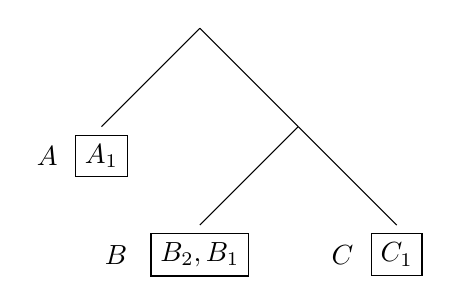
\begin{tikzpicture}[scale = 1.25]
            \node[draw, align=left] at (-1,-1.3) {$A_1$};
            \node[align=left] at (-1.55,-1.3) {$A$};
            \node[draw, align=left] at (0,-2.3) {$B_2, B_1$};
            \node[align=left] at (-0.85,-2.3) {$B$};
            \node[draw, align=left] at (2,-2.3) {$C_1$};
            \node[align=left] at (1.45,-2.3) {$C$};
            
            \draw (0,0) -- (-1, -1);
            \draw (0,0) -- (1, -1);
            \draw (1,-1) -- (0, -2);
            \draw (1,-1) -- (2, -2);
        \end{tikzpicture}
        \caption{Over topology $\Node(\ast, \Node(\ast, \ast))$}
    \end{subfigure}
    \begin{subfigure}[t]{0.49\linewidth}
        \centering
        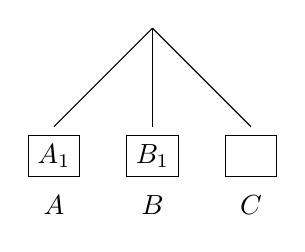
\begin{tikzpicture}[scale = 1.25]
            \node[draw, align=left] at (-1,-1.3) {$A_1$};
            \node[draw, align=left] at (0,-1.3) {$B_1$};
            \node[draw, align=left] at (1,-1.3) {\phantom{$C_1$}};
            \node[align=left] at (-1,-1.8) {$A$};
            \node[align=left] at (0,-1.8) {$B$};
            \node[align=left] at (1,-1.8) {$C$};

            \draw (0,0) -- (-1, -1);
            \draw (0,0) -- (0, -1);
            \draw (0,0) -- (1, -1);
        \end{tikzpicture}
        \caption{Over topology $\Node(\ast, \ast, \ast)$}
    \end{subfigure}
    \caption{Rio trees decorated by classes $A$, $B$, and $C$}
\end{figure}

\begin{dfn}
    For topology $t \in \Topo$, the set $\RioTree(t)$ of \emph{Rio trees} over $t$ is defined by
    \begin{align*}
        \inference{}
        {p \in \PIFO(\Pkt)\\ c \in \Class}
        {\Leaf(p, c) \in \RioTree(\ast)}
        &&
        \inference{}
        {
            ts \in \Topo^n\\
            \forall 1 \leq i \leq n. \; qs[i] \in \RioTree(ts[i])
        }
        {\Internal(qs) \in \RioTree(\Node(ts))}
    \end{align*}
    These are trees with leaves decorated by both classes and PIFOs.
\end{dfn}

\begin{dfn}
    For topology $t \in \Topo$, the set $\OrdTree(t)$ of \emph{ordered trees} over $t$ is defined by
    \begin{align*}
        \axiom{}
        {\Leaf \in \OrdTree(\ast)}
        &&
        \inference{}
        {
            ts \in \Topo^n\\
            rs \in \Rk^{n}\\\\
            \forall 1 \leq i < j \leq n. \; rs[i] \neq rs[j]\\
            \forall 1 \leq i \leq n. \; os[i] \in \OrdTree(ts[i])
        }
        {\Internal(rs, os) \in \OrdTree(\Node(ts))}
    \end{align*}
    These are trees with each internal node's child given a \emph{unique} rank, thereby inducing a total ordering of children.
\end{dfn}

Let $\flow : \Pkt \to \Class$ be an opaque mapping from packets to the class they belong to (flow inference).

\begin{dfn}
    For $t \in \Topo$, define $\push : \RioTree(t) \times \Pkt \times \Rk \halfto \RioTree(t)$ such that
    \begin{align*}
        \inference{}
        {
            \flow(\pkt) = c\\
            \push(p, \pkt, r) = p^\prime
        }
        {\push(\Leaf(p, c), \pkt, r) = \Leaf(p^\prime, c)}
        &&
        \inference{}
        {
            \forall 1 \leq i \leq |qs|. \; \push(qs[i], \pkt, r) = qs^\prime[i]
        }
        {\push(\Internal(qs), \pkt, r) = \Internal(qs^\prime)}
        &&
        \inference{}
        {
            \flow(\pkt) \neq c\\
        }
        {\push(\Leaf(p, c), \pkt, r) = \Leaf(p, c)}
    \end{align*}
    Informally, we recursively push to all subtrees but only the PIFOs on leaves with the packet's flow are updated.
\end{dfn}

\begin{dfn}
    For $t \in \Topo$, define $\pop : \RioTree(t) \times \OrdTree(t) \halfto \Pkt \times \RioTree(t)$ such that
    \begin{align*}
        \inference{}
        {\pop(p) = (\pkt, p^\prime)}
        {\pop(\Leaf(p, c), \Leaf) = (\pkt, \Leaf(p^\prime, c))}
        &&
        \inference{}
        {
            \pop(qs[i], os[i]) = (\pkt, q)\\\\
            \forall 1 \leq j \leq |qs|. \; j \neq i \land \pop(qs[j], os[j]) = (\pkt^\prime, q^\prime) \implies rs[i] < rs[j]
        }
        {\pop(\Internal(qs), \Internal(rs, os)) = (\pkt, \Internal(qs[q/i]))}
    \end{align*}
    Informally, we recursively pop the smallest ranked, poppable subtree.
\end{dfn}

\section{Modelling Scheduling Algorithms}

Like \cite{OG}, we model scheduling algorithms through a \emph{control}, a thin-layer over the tree policies run on.
They keep track of 
\begin{enumerate}
    \item a state from a fixed collection $\St$
    \item an underlying tree of buffered packets % is buffered the right word?
    \item scheduling transactions that update state and construct auxillary structures to push or pop the tree
\end{enumerate}
They come in two flavors: Rio \& PIFO Controls.
The former determines the order to forward packets at dequeue while latter does so at enqueue.

\subsection{Controls}

\begin{figure}[!htb]
    \begin{align*}
        &\inference{RioCtrl-Push}
        {
            \zprepush(s, \pkt) = (r, s^\prime)\\
            \push(q, \pkt, r) = q^\prime
        }
        {
            \push((s, q, \zprepush, \zprepop, \zpostpop), \pkt) 
            = 
            (s^\prime, q^\prime, \zprepush, \zprepop, \zpostpop)
        }\\
        &\inference{RioCtrl-Pop}
        {
            \zprepop(s) = (o, s^\prime)\\
            \pop(q, o) = (\pkt, q^\prime)\\
            \zpostpop(s^\prime, \pkt) = s^{\prime\prime}
        }
        {
            \pop((s, q, \zprepush, \zprepop, \zpostpop)) 
            = 
            (\pkt, (s^{\prime\prime}, q^\prime, \zprepush, \zprepop, \zpostpop))
        }\\
        &\inference{PIFOCtrl-Push}
        {
            \zprepush(s, \pkt) = (pt, s^\prime)\\
            \push(q, \pkt, pt) = q^\prime
        }
        {
            \push((s, q, \zprepush, \zpostpop), \pkt) 
            = 
            (s^\prime, q^\prime, \zprepush, \zpostpop)
        }\\
        &\inference{PIFOCtrl-Pop}
        {
            \pop(q) = (\pkt, q^\prime)\\
            \zpostpop(s, \pkt) = s^\prime
        }
        {
            \pop((s, q, \zprepush, \zpostpop)) 
            = 
            (\pkt, (s^\prime, q^\prime, \zprepush, \zpostpop))
        }
    \end{align*}
    \caption{Pushing and Popping Controls}
    \label{fig:control_push_pop}
\end{figure}

\begin{dfn}
    Let $t \in \Topo$ and \emph{scheduling transactions} $\zprepush$ and $\zpostpop$ be partial functions
    \begin{align*}
        \zprepush &: \St \times \Pkt \halfto \Path(t) \times \St\\
        \zpostpop &: \St \times \Pkt \halfto \St
    \end{align*}
    Define $\PIFOControl(t, \zprepush, \zpostpop)$ to be the set of quadruples 
    $$(s, q, \zprepush, \zpostpop)$$
    where $s \in \St$ and well-formed $q \in \PIFOTree(t)$.
\end{dfn}

\begin{dfn}
    Let $t \in \Topo$ and \emph{scheduling transactions} $\zprepush, \zprepop, \zpostpop$ be partial functions
    \begin{align*}
        \zprepush &: \St \times \Pkt \halfto \Rk \times \St\\
        \zprepop  &: \St \halfto \OrdTree(t) \times \St\\
        \zpostpop &: \St \times \Pkt \halfto \St
    \end{align*}
    Define $\RioControl(t, \zprepush, \zprepop, \zpostpop)$ to be the set of quintuples 
    $$(s, q, \zprepush, \zprepop, \zpostpop)$$ 
    where $s \in \St$ and $q \in \RioTree(t)$.
\end{dfn}

Both controls admit $\push$ and $\pop$ operations:
\begin{align*}
    \push &: \PIFOControl(t, \zprepush, \zpostpop) \times \Pkt \halfto \PIFOControl(t, \zprepush, \zpostpop)\\
    \pop  &: \PIFOControl(t, \zprepush, \zpostpop) \halfto \Pkt \times \PIFOControl(t, \zprepush, \zpostpop)\\
    \push &: \RioControl(t, \zprepush, \zprepop, \zpostpop) \times \Pkt \halfto \RioControl(t, \zprepush, \zprepop, \zpostpop)\\
    \pop  &: \RioControl(t, \zprepush, \zprepop, \zpostpop) \halfto \Pkt \times \RioControl(t, \zprepush, \zprepop, \zpostpop)
\end{align*}

Their semantics are written out in full in \Cref{fig:control_push_pop}.

\subsection{Simulations}

\begin{dfn}
    \label{dfn:empty}
    For $t \in \Topo$, define $\emt_t \in \PIFOTree(t)$ such that
    \begin{align*}
        \inference{}
        {p \in \PIFO(\Pkt)\\ \pop(p) \text{ is undefined}}
        {\emt_{\ast} = \Leaf(p)}
        &&
        \inference{}
        {
            ts \in \Topo^n\\
            p \in \PIFO(\{1, \ldots, n\})\\\\
            \pop(p) \text{ is undefined}\\
            \forall 1 \leq i \leq n. \; qs[i] = \emt_{ts[i]}
        }
        {\emt_{\Node(ts)} = \Internal(p, qs)}
    \end{align*}
    Informally, $\emt_t$ is a PIFO tree of topology $t$, with empty PIFOs at all nodes.
\end{dfn}

\begin{dfn}
    \label{dfn:step}
    Define the $\to \; \subseteq \PIFOControl(t, \zprepush, \zpostpop) \times \PIFOControl(t, \zprepush, \zpostpop)$ by
    \begin{align*}
        \inference{Step-Push}
        {\pkt \in \Pkt\\ \push(c, \pkt) = c^\prime}
        {c \to c^{\prime}}
        &&
        \inference{Step-Pop}
        {\pop(c) = (\pkt, c^\prime)}
        {c \to c^{\prime}}
    \end{align*}
    i.e. $c \to c^\prime$ if $c^\prime$ is a push or pop from $c$.
    We write $\to^\ast$ for the reflexive transitive closure of $\to$.
\end{dfn}

\begin{dfn}
    A partial function
    $$
        f :  
        \PIFOControl(t, \zprepush, \zpostpop) 
        \halfto
        \RioControl(t^\prime, \tzprepush, \tzprepop, \tzpostpop) 
    $$
    is \emph{simulation} if the following conditions are satisfied:
    \begin{enumerate}
        \item There exists $\cinit = (s, q, \zprepush, \zpostpop)$ where $q = \emt_t$ and $\cinit \in \operatorname{dom} f$.
        \item When $\cinit \to^\ast c_1$ and $f(c_1) = c_2$, we can guarantee the following:
            \begin{align}
                \pop(c_1) \text{ is undefined} &\implies \pop(c_2) \text{ is undefined}\\
                \pop(c_1) = (\pkt, c^\prime_1) &\implies \pop(c_2) = (\pkt, c^\prime_2) \land f(c_1^\prime) = c_2^\prime\\
                \push(c_1, \pkt) = c^\prime_1  &\implies \push(c_2, \pkt) = c^\prime_2 \land f(c_1^\prime) = c_2^\prime
            \end{align}
    \end{enumerate}
\end{dfn}


\newpage

\section{Example Controls \& Simulations}

All further discussion takes $\St = \text{set of dictionaries mapping $\textbf{string} \to \textbf{float}$}$ and $\Rk = \Class = \mathbb N$.

\subsection{Round-Robin}

\begin{figure}[!htb]
    \centering
    \begin{subfigure}[t]{0.49\linewidth}
        \lstinputlisting{sched_trans/pifo/z_pre-push.pseudo}
        \lstinputlisting{sched_trans/pifo/z_post-pop.pseudo}
        \caption{Round-Robin PIFO Control}
        \label{fig:rr-pifo-ctrl}
    \end{subfigure}
    \begin{subfigure}[t]{0.49\linewidth}
        \lstinputlisting{sched_trans/rio/z_pre_push.pseudo}
        \lstinputlisting{sched_trans/rio/z_pre-pop.pseudo}
        \lstinputlisting{sched_trans/rio/z_post-pop.pseudo}
        \caption{Round-Robin Rio Control}
        \label{fig:rr-rio-ctrl}
    \end{subfigure}
    \caption{Scheduling Transactions}
    \label{fig:sched_trans}
\end{figure}

For $n \in \mathbb N$, let's put our theory to use by constructing PIFO and Rio controls for
\begin{align*}
    \RR[(\FIFO[0], \FIFO[1], \ldots, \FIFO[n - 1])] 
\end{align*}

Both controls use the same underlying topology, namely
$$
t = \Node(\underbrace{\ast, \ast, \ldots, \ast}_{n \text{ times}})
$$
\Cref{fig:sched_trans} describes their scheduling transactions in pseudocode.
Therefore, we have the materials to define
\begin{align*}
    \PIFOControl(t, \zprepush, \zpostpop)
    &&
    \text{and}
    &&
    \RioControl(t, \tzprepush, \tzprepop, \tzpostpop)
\end{align*}
I.e. the collection of PIFO and Rio controls for our program.
Let's find a simulation between them!

\begin{dfn}
    \label{dfn:rrinit}
    Let $\crr = (s, \emt_t, \zprepush, \zpostpop) \in \PIFOControl(t, \zprepush, \zpostpop)$, where
    \begin{align*}
        s[``\text{counter}"] = 0 &&
        s[``\text{turn}"] = 0 &&
        s[``\text{cycle}"] = 1 &&
        s[``r\_" + \text{str}(i)] = i 
    \end{align*}
    for all $0 \leq i \leq n - 1$
\end{dfn}

\begin{dfn}
    \label{dfn:ranks}
    For set $S$, define $\ranks : \PIFO(S) \times S \to \mathcal M(\Rk)$\footnote{
        We use $\mathcal M(X)$ to denote the collection of \href{https://en.wikipedia.org/wiki/Multiset}{multisets} with entries in set $X$.
    } 
    such that
    \begin{align*}
        \inference{}
        {\pop(p^\prime) = (j, p)\\ m = \min(\ranks(p^\prime, j))\\ i = j}
        {\ranks(p, i) = \ranks(p^\prime, i) - \{m\}}
        \hspace{10mm}
        \inference{}
        {\pop(p^\prime) = (j, p)\\ i \neq j}
        {\ranks(p) = \ranks(p^\prime, i)}
        \\
        \inference{}
        {\push(p^\prime, j, r) = p\\ i = j}
        {\ranks(p, i) = \ranks(p^\prime, i) + \{r\}}
        \hspace{5mm}
        \inference{}
        {\pop(p) \text{ is undefined}}
        {\ranks(p, i) = \{\}}
        \hspace{5mm}
        \inference{}
        {\push(p^\prime, j, r) = p\\ i \neq j}
        {\ranks(p, i) = \ranks(p^\prime, i)}
    \end{align*}
    Informally, $\ranks(p, i)$ is the multiset of ranks with which $i$ lives in PIFO $p$.
\end{dfn}

\begin{lem}
    \label{lem:ranks}
    If $\crr \to^\ast c = (s, q, \zprepush, \zpostpop)$ and $p$ is $q$'s root PIFO, i.e. $q = \Internal(p, qs)$, then
    $$
        \ranks(p, i) =
        \begin{cases}
            \Big\{x \in \Rk \mid x \equiv i \pmod n \land n \cdot s[``\text{cycle}"] \leq x < s[``r\_" + \mathrm{str}(i)] \Big\} 
            & i < s[``\text{turn}"]\\
            \Big\{x \in \Rk \mid x \equiv i \pmod n \land n \cdot (s[``\text{cycle}"] - 1) \leq x < s[``r\_" + \mathrm{str}(i)]\Big\} 
            & i \geq s[``\text{turn}"]
        \end{cases}
    $$
    for all $0 \leq i \leq n - 1$.
\end{lem}

\begin{proof}
    We'll proceed by induction on $\to^\ast$.
    \begin{enumerate}
        \item[(Base Case)] Let $c = \crr$ and fix arbitrary $i \in [0, n - 1]$.\\
            Recall $q = \emt_t$ by \Cref{dfn:rrinit}. 
            Therefore, $\pop(p)$ is undefined by \Cref{dfn:empty}.
            Hence, $$\ranks(p, i) = \{\}$$ by \Cref{dfn:ranks}.
            \Cref{dfn:rrinit} also insists
            \begin{align*}
                s[``\text{turn}"] = 0
                &&
                s[``cycle"] = 1
                &&
                s[``r\_" + str(i)] = i
            \end{align*}
            Hence, $i \geq s[``\text{turn}"]$ and
            \begin{align*}
                &=
                \begin{cases}
                    \Big\{x \in \Rk \mid x \equiv i \pmod n \land n \cdot s[``cycle"] \leq x < s[``r\_" + \mathrm{str}(i)] \Big\} 
                    & i < s[``\text{turn}"]\\
                    \Big\{x \in \Rk \mid x \equiv i \pmod n \land n \cdot (s[``cycle"] - 1) \leq x < s[``r\_" + \mathrm{str}(i)]\Big\} 
                    & i \geq s[``\text{turn}"]
                \end{cases}\\
                &= \Big\{x \in \Rk \mid x \equiv i \pmod n \land n \cdot (s[``cycle"] - 1) \leq x < s[``r\_" + \mathrm{str}(i)]\Big\}\\
                &= \Big\{x \in \Rk \mid x \equiv i \pmod n \land 0 \leq x < i \Big\} = \{\}
            \end{align*}
            Both sides of the desired equality are therefore the empty multiset $\{\}$.
        \item[(Inductive Step)] Let $c^\prime = (s^\prime, q^\prime, \zprepush, \zpostpop) \to c$ and $q^\prime = \Internal(p^\prime, qs^\prime)$.
            We have two cases.
            \begin{enumerate}
                \item[(Step-Push)] Suppose $c = \push(c^\prime, \pkt)$ and $f = \flow(\pkt)$.
                    From inspecting $\zprepush$ in \Cref{fig:rr-pifo-ctrl},
                    \begin{align*}
                        \push\Big(p^\prime, f, s^\prime[``r\_" + \mathrm{str}(f)]\Big) = p
                        &&
                        s[x] =
                        \begin{cases}
                            s^\prime[x] + n & x = ``r\_" + \mathrm{str}(f)\\
                            s^\prime[x] + 1 & x = ``\text{counter}"\\
                            s^\prime[x] & \text{otherwise}
                        \end{cases}
                    \end{align*}
                    Hence, by \Cref{dfn:ranks} and the IH, for $i \neq f$,
                    \begin{align*}
                        &= \ranks(p, i) = \ranks(p^\prime, i)\\
                        &=
                            \begin{cases}
                                \Big\{x \in \Rk \mid x \equiv i \pmod n \land n \cdot s^\prime[``cycle"] \leq x < s^\prime[``r\_" + \mathrm{str}(i)] \Big\} 
                                & i < s^\prime[``\text{turn}"]\\
                                \Big\{x \in \Rk \mid x \equiv i \pmod n \land n \cdot (s^\prime[``cycle"] - 1) \leq x < s^\prime[``r\_" + \mathrm{str}(i)]\Big\} 
                                & i \geq s^\prime[``\text{turn}"]
                            \end{cases}\\
                        &=
                            \begin{cases}
                                \Big\{x \in \Rk \mid x \equiv i \pmod n \land n \cdot s[``cycle"] \leq x < s[``r\_" + \mathrm{str}(i)] \Big\} 
                                & i < s[``\text{turn}"]\\
                                \Big\{x \in \Rk \mid x \equiv i \pmod n \land n \cdot (s[``cycle"] - 1) \leq x < s[``r\_" + \mathrm{str}(i)]\Big\} 
                                & i \geq s[``\text{turn}"]
                            \end{cases}
                    \end{align*}
                    Instead, for $i = f$, let $r = s^\prime[``r\_" + \mathrm{str}(i)]$. 
                    \Cref{dfn:ranks} and the IH then once again show
                    \begin{align*}
                        &= \ranks(p, i) = \ranks(p^\prime, i) + \{r\}\\
                        &=
                            \begin{cases}
                                \Big\{x \in \Rk \mid x \equiv i \pmod n \land n \cdot s^\prime[``cycle"] \leq x < s^\prime[``r\_" + \mathrm{str}(i)] \Big\} + \{r\}
                                & i < s^\prime[``\text{turn}"]\\
                                \Big\{x \in \Rk \mid x \equiv i \pmod n \land n \cdot (s^\prime[``cycle"] - 1) \leq x < s^\prime[``r\_" + \mathrm{str}(i)]\Big\} + \{r\}
                                & i \geq s^\prime[``\text{turn}"]
                            \end{cases}\\
                        &=
                            \begin{cases}
                                \Big\{x \in \Rk \mid x \equiv i \pmod n \land n \cdot s^\prime[``cycle"] \leq x < s^\prime[``r\_" + \mathrm{str}(i)] + n\Big\}
                                & i < s^\prime[``\text{turn}"]\\
                                \Big\{x \in \Rk \mid x \equiv i \pmod n \land n \cdot (s^\prime[``cycle"] - 1) \leq x < s^\prime[``r\_" + \mathrm{str}(i)] + n\Big\}
                                & i \geq s^\prime[``\text{turn}"]
                            \end{cases}\\
                        &=
                            \begin{cases}
                                \Big\{x \in \Rk \mid x \equiv i \pmod n \land n \cdot s[``cycle"] \leq x < s[``r\_" + \mathrm{str}(i)] \Big\}
                                & i < s[``\text{turn}"]\\
                                \Big\{x \in \Rk \mid x \equiv i \pmod n \land n \cdot (s[``cycle"] - 1) \leq x < s[``r\_" + \mathrm{str}(i)]\Big\}
                                & i \geq s[``\text{turn}"]
                            \end{cases}
                    \end{align*}

                \item[(Step-Pop)] Suppose $(\pkt, c) = \pop(c^\prime)$ and $f = \flow(\pkt)$. 
                    From inspecting $\zpostpop$ in \Cref{fig:rr-pifo-ctrl},
                    \begin{align*}
                        \pop(p^\prime) = (f, p) %This claim maybe requires proof; definitely true though
                        &&
                        s[``\text{cycle}"] \in \{s^\prime[``\text{cycle}"], s^\prime[``\text{cycle}"] + 1\}
                    \end{align*}
                    Consider the case where $s[``\text{cycle}"] = s^\prime[``\text{cycle}"]$, i.e. $s^\prime[``\text{turn}"] \leq f < s[``\text{turn}"] = f + 1$.
                    \begin{itemize}
                        \item For $i < s^\prime[``\text{turn}"]$ or $i \geq s[``\text{turn}"]$, lines 5-7 of $\zpostpop$ in \Cref{fig:rr-pifo-ctrl} show
                            $$s[``r\_" + \mathrm{str}(i)] = s^\prime[``r\_" + \mathrm{str}(i)]$$
                            Therefore, by \Cref{dfn:ranks} and the IH,
                            \begin{align*}
                                &= \ranks(p, i) = \ranks(p^\prime, i)\\
                                &=
                                    \begin{cases}
                                        \Big\{x \in \Rk \mid x \equiv i \pmod n \land n \cdot s^\prime[``cycle"] \leq x < s^\prime[``r\_" + \mathrm{str}(i)] \Big\} 
                                        & i < s^\prime[``\text{turn}"]\\
                                        \Big\{x \in \Rk \mid x \equiv i \pmod n \land n \cdot (s^\prime[``cycle"] - 1) \leq x < s^\prime[``r\_" + \mathrm{str}(i)]\Big\} 
                                        & i \geq s^\prime[``\text{turn}"]
                                    \end{cases}\\
                                &=
                                    \begin{cases}
                                        \Big\{x \in \Rk \mid x \equiv i \pmod n \land n \cdot s[``cycle"] \leq x < s[``r\_" + \mathrm{str}(i)] \Big\} 
                                        & i < s[``\text{turn}"]\\
                                        \Big\{x \in \Rk \mid x \equiv i \pmod n \land n \cdot (s[``cycle"] - 1) \leq x < s[``r\_" + \mathrm{str}(i)]\Big\} 
                                        & i \geq s[``\text{turn}"]
                                    \end{cases}
                            \end{align*}

                        \item For $s^\prime[``turn"] \leq i < f$, lines 5-7 of $\zpostpop$ in \Cref{fig:rr-pifo-ctrl} show
                            $$s[``r\_" + \mathrm{str}(i)] = s^\prime[``r\_" + \mathrm{str}(i)] + n$$
                            and the IH says
                            \begin{align*}
                                \ranks(p^\prime, i) &= 
                                \Big\{x \in \Rk \mid x \equiv i \pmod n \land n \cdot (s^\prime[``cycle"] - 1) \leq x < s^\prime[``r\_" + \mathrm{str}(i)]\Big\}\\
                                \ranks(p^\prime, f) &= 
                                \Big\{x \in \Rk \mid x \equiv f \pmod n \land n \cdot (s^\prime[``cycle"] - 1) \leq x < s^\prime[``r\_" + \mathrm{str}(f)]\Big\} 
                            \end{align*}
                            Since popping $p^\prime$ returned $f$, it must be a minimally ranked element.
                            However,
                            $$
                                n \cdot (s^\prime[``cycle"] - 1) + i
                                < 
                                n \cdot (s^\prime[``cycle"] - 1) + f
                            $$
                            Therefore, $\ranks(p^\prime, i) = \{\}$:
                            i.e. there are no numbers congruent to $i \mod n$ in
                            $$
                                \Big[n \cdot (s^\prime[``cycle"] - 1), s^\prime[``r\_" + \mathrm{str}(i)]\Big)
                            $$
                            The same is therefore true of
                            $$
                                \Big[n \cdot s^\prime[``cycle"], s^\prime[``r\_" + \mathrm{str}(i)] + n\Big)
                            $$
                            Putting all this together with \Cref{dfn:ranks},
                            \begin{align*}
                                &= \ranks(p, i) = \ranks(p^\prime, i)\\
                                &=
                                \Big\{x \in \Rk \mid x \equiv i \pmod n \land n \cdot (s^\prime[``cycle"] - 1) \leq x < s^\prime[``r\_" + \mathrm{str}(i)]\Big\}\\
                                &= \{\}\\
                                &=
                                \Big\{x \in \Rk \mid x \equiv i \pmod n \land n \cdot s^\prime[``cycle"] \leq x < s^\prime[``r\_" + \mathrm{str}(i)] + n\Big\}\\
                                &=
                                    \begin{cases}
                                        \Big\{x \in \Rk \mid x \equiv i \pmod n \land n \cdot s[``cycle"] \leq x < s[``r\_" + \mathrm{str}(i)] \Big\} 
                                        & i < s[``\text{turn}"]\\
                                        \Big\{x \in \Rk \mid x \equiv i \pmod n \land n \cdot (s[``cycle"] - 1) \leq x < s[``r\_" + \mathrm{str}(i)]\Big\} 
                                        & i \geq s[``\text{turn}"]
                                    \end{cases}
                            \end{align*}

                        \item For $i = f$, lines 5-7 of $\zpostpop$ in \Cref{fig:rr-pifo-ctrl} yet again show
                            $$s[``r\_" + \mathrm{str}(i)] = s^\prime[``r\_" + \mathrm{str}(i)]$$
                            and the IH says
                            $$
                                \ranks(p^\prime, i) = 
                                \Big\{x \in \Rk \mid x \equiv i \pmod n \land n \cdot (s^\prime[``\text{cycle}"] - 1) \leq x < s^\prime[``r\_" + \mathrm{str}(i)]\Big\} 
                            $$
                            By \Cref{dfn:ranks},
                            \begin{align*}
                                &= \ranks(p, i) = \ranks(p^\prime) - \{n \cdot (s^\prime[``\text{cycle}"] - 1)\}\\
                                &= \Big\{x \in \Rk \mid x \equiv i \pmod n \land n \cdot s^\prime[``\text{cycle}"] \leq x < s^\prime[``r\_" + \mathrm{str}(i)]\Big\}\\
                                &= \Big\{x \in \Rk \mid x \equiv i \pmod n \land n \cdot s[``\text{cycle}"] \leq x < s[``r\_" + \mathrm{str}(i)]\Big\}\\
                                &=
                                    \begin{cases}
                                        \Big\{x \in \Rk \mid x \equiv i \pmod n \land n \cdot s[``cycle"] \leq x < s[``r\_" + \mathrm{str}(i)] \Big\} 
                                        & i < s[``\text{turn}"]\\
                                        \Big\{x \in \Rk \mid x \equiv i \pmod n \land n \cdot (s[``cycle"] - 1) \leq x < s[``r\_" + \mathrm{str}(i)]\Big\} 
                                        & i \geq s[``\text{turn}"]
                                    \end{cases}
                            \end{align*}
                    \end{itemize}
            \end{enumerate}
    \end{enumerate}
\end{proof}

\newpage

\subsection{Strict}

\newpage

\renewcommand\refname{\LARGE References}
\bibliographystyle{alpha}
\bibliography{refs}

\end{document}
